\chapter{Practical Appliance}
As described in the previous chapter, this one will walk through the requirement engineering process for a B2B marketing application. A label based on a capital letter and a hierarchical number will be used for itemized \mbox{information (\textbf{I})}, \mbox{requirements (\textbf{R})} (e.g. \ssay{\textbf{I3.2.3}}).
\section{Input information}
\subsection{The Sponsor}
The sponsor, he explained, that he would like to have an application or website, which he "can give to a customer to play around with and get to know the skills of IBM" \parencite{Sachs.20.04.2017b}. As a legacy from times when IBM was mainly a mainframe hardware supplier, IBM is perceived with its past skill , he further points out \parencite{Sachs.20.04.2017b}. Therefore the app must arouse the interest of the potential customer and display that IBM has experience, knowledge and skills in the domain of banking software migration. 

\paragraph{} As a condition for access by the potential customer, the sponsor required some kind of authentication, which would lock the customer out after two weeks time, if the access is not extended by an IBM opportunity owner.

\paragraph{} 'Opportunity owner' in this thesis refers to the responsible employee for a opportunity to sell IBM services.

\paragraph{} As a visual appearance, the sponsor demanded a stereotypical generalized online banking application.

Constraining the development of the application, the sponsor requested that the application will not generate costs when not in use, is developed by corporate student in their three month practical - as it is common at IBM - and will be developed in iterative development \textbf{cycles}. This approach is requested to ensure usable products after the three month term.

\paragraph{} Summarized:

\begin{closeItem}
    \item [\textbf{I1}] When a customer uses the application, the system shall provide him with the ability to receive information about IBM skills.
    \item [\textbf{I2}] When a customer tries to use the site, the system shall request some kind of authentication.
    \item [\textbf{I2.1}] When customer access rights age two weeks without being extended, the system shall revoke the access rights.
    \item [\textbf{I2.2}\label{R2.2}] When a user is an opportunity owner of IBM the application, the system shall provide the user with the ability to extend customer access rights.
    \item [\textbf{I3}] The system shall superficially appear like a mobile online banking application.
\end{closeItem}

\paragraph{} It is implied by \textbf{I2.2}, that IBM opportunity owner must be able to log into the system in a way that proves their employment status at IBM. This causes a new Requirement:

\begin{closeItem}
    \item [\textbf{I4}] When the system is accessed, it shall provide IBM opportunity owners the ability to log in with their corporate identity.
\end{closeItem}

\subsection{Organizational Standards}
Subsequent to \textbf{I4}, IBM has a organizational standard for authentication on application, which are also available online: the so-called w3ID-Log in \parencite[cf.][]{IBMCorporation.2016}.

\begin{closeItem}
    \item [\textbf{I4.1}] When a user wants to identify as an IBM opportunity owner, the system shall utilize w3ID for authentication.
\end{closeItem}

\paragraph{} In addition to authentication procedures, IBM requires all applications to follow a set of rules:

\paragraph{} The development must follow the 'MobileFirst'-idea, if applicable \parencite[cf.][]{IBMCorporation.2016}. This is explained as acting on the principle to develop everything for mobile devices first. That of course only applies only on applications intended for use on mobile devices.

\paragraph{} Mobile device referes to small screen devices with no keyboard in this context \parencite[cf.][]{Duong.2014}. Afterwards the design and functionality may be extended to larger devices with more peripheral devices (mouse, keyboard, etc.) and larger screens.

\paragraph{} The application, to this point, do not show any reason to not be available on mobile device, therefore:

\begin{closeItem}
    \item [\textbf{I5}] When a developer does work for the system, the developer should do the work for mobile devices prioritized.
\end{closeItem}

\subsection{Regulations}
No proof could be found for any regulation concerning the functionality of the application. To this point, it will not collect any information, display any personal information, export US-American intellectual property or show any other regulation related behaviour. On the other hand, this research must be done exhaustively by a legal expert, which was not available for this research.

\subsection{Domain Information}
The domain of B2B marketing is described in \Cref{} on \cpagerefrange{}{}. Important conclusions are: 

\begin{closeItem}
    \item [\textbf{I6}] When creating the stakeholder map, the requirements engineer shall integrate the customer's stakeholders.
    \item [\textbf{I7}] When a B2B customer is approached, the communication should address to his or her individual case.
\end{closeItem}

Since the principle of attention economy suggests that attention of users may be lost quickly due to other factors (cf. \Cref{}):

\begin{closeItem}
    \item [\textbf{I8}] When a customer stops using the application, the application should be able to retrieve his or her attention.
\end{closeItem}

\paragraph{}

\subsection{Stakeholder Needs}
As described earlier, in order to identify stakeholder need, the stakeholders must be identified. Firstly, all stakeholder which were directly mentioned to this point can be identified:

\begin{closeItemCol}
    \item customer (\textbf{I1})
    \item sponsor
    \item IBM opportunity owner (\textbf{I2.2})
    \item IBM Corporation
    \item developer (\textbf{I5})
\end{closeItemCol}

The sponsor and IBM corporation are not tracked back, since they are the basic setting for the research.

\paragraph{} These stakeholders are pretty vague. Who is the \ssay{customer}. Deriving from the sponsors information, that the application should be handed to the customer during a bidding procedure as result of a call for proposal, the author deduces based on past experience that the \ssay{customer} can either be the procurement of the calling company, the future steering committee of the to-be project naming the management of the demanding company. 

\paragraph{} This leads to the \ssay{customer} to be subdivided. The sponsor, the opportunity owner and the contributor can all be classified as IBM employee.

\begin{closeItemCol}
    \item customer (\textbf{I1})
    \begin{itemize}
        \item procurement officer
        \item operational manager
        \item IT department representative
        \item legal and compliance advisor
        \item finance representative
    \end{itemize} \columnbreak
    
    \item IBM employee 
    \begin{itemize}
        \item sponsor
        \item developer (\textbf{I5})
        \item opportunity owner (\textbf{I2.2})
    \end{itemize}
    \item IBM Corporation
\end{closeItemCol}

In reference to the specialties of B2B marketing mentioned on \cpageref{}, the customer demand for service is only derived from their customer demands. Therefore, these customers have to be included as well. 

\paragraph{} Basically, those can be separated into consumers and other businesses. As of the explanation from the sponsor, the consumer group is split into 2 groups: core banking customer, meaning people who only have bank account and credits, and those who additionally do stock broking. 

\paragraph{} Same is somehow true for B2B clients, but those are much more diverse than consumers. They may have individual terms and conditions, distribute stocks and so on. 

\paragraph{} For simplicity, we regard consumers and companies as equal as long as the diversity does not have an impact.

\paragraph{}
Regarding the professional context of a bank, it becomes clear that two of their stakeholder are of special importance: Firstly, the stock brokers require tax statements by the bank, which are critical for the banks clients annual tax declaration. Secondly, the \ssay{Bundesanstalt für 
Finanzdienstleistungsaufsicht} (BaFin), the German institute for financial supervision, requires notes on a regular basis from the bank.

\begin{closeItem}
    \item [\textbf{I9}] When information is collected for the application, the creators should not forget the regular notes to the BaFin.
    \item [\textbf{I10}] When information is collected for the application, the creators should not forget about stock trading tax issues.
\end{closeItem}

\vspace{2em}


\begin{closeItemCol}
    \NoIndent{\textbf{IBM's stakeholders:}}
    \item customer (\textbf{I1})
    \begin{itemize}
        \item procurement officer
        \item operational manager
        \item IT department representative
        \item legal and compliance advisor
        \item finance representative
    \end{itemize}
    \item IBM employee 
    \begin{itemize}
        \item sponsor
        \item developer (\textbf{I5})
        \item opportunity owner (\textbf{I2.2})
    \end{itemize}
    \item IBM Corporation
    \columnbreak
    \NoIndent{\textbf{Stakeholders of the customer:}}
    \item BaFin
    \item stock broker
    \item core banking customers
\end{closeItemCol}

\subsubsection{Stakeholder Maps}
For translation into stakeholder maps as described in \Cref{} on \cpageref{}, the stakeholders must be ordered by intensity of usage, and by influence on the service. Each from the perspective of the service. Therefore the stakeholders of IBM will be ordered by the usage and influence of the desired marketing app, and the customer's stakeholders by the usage of and influence on the banking service.

\paragraph{}
Ordering the IBM's stakeholders by usage is pretty straight foreword: The IBM opportunity owners will be the most frequent users, because they will use the application frequently to allow customer access. All customer roles will be using the application for a single approximately two week time period what makes them irregular users.
The developer and IBM Corporation will not be users of the application, one only accessing the application for test reasons, the other executing only regulatory authority. 

\paragraph{} More carefully, the order of influence must be generated, since the term influence can be ambiguous: On the one hand, it could mean the influence on the app development - which is the correct interpretation (cf. \Cref{}) -, on the other hand, the influence on the buying decision of the customer might be of interest.


\begin{figure}[H]
    \centering
    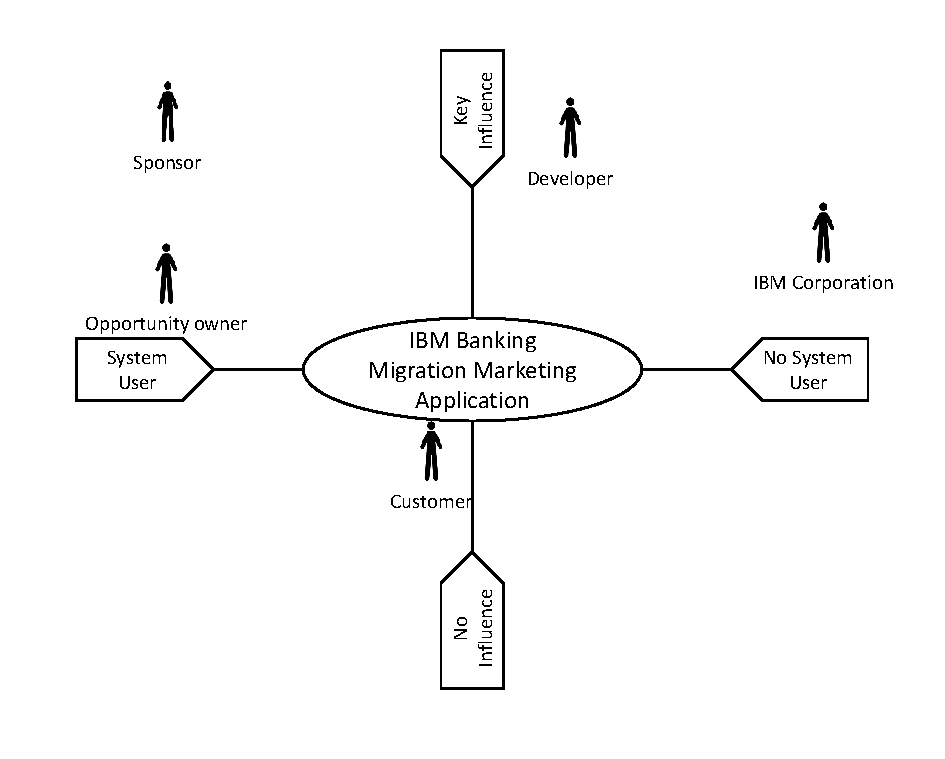
\includegraphics[height=.5\textheight]{img/smMarketingApp.pdf}
    \caption[Stakeholder Map of IBM Marketing Application]{Stakeholder Map of IBM Marketing Application (own illustration)}
    \label{fig:smIBM}
\end{figure}

As to be seen in \Cref{fig:smIBM} the order in influence was decided to be in the following order: The sponsor being most influential, since he is supervising the application life cycle from the conception via development to deployment and can empower influence at any time. Secondly, the developer has got great impact on the application, because his skills and commitment shape the application. Thirdly, the IBM Cooperation influences the application by requiring certain development and style guidelines. At fourth position come the opportunity owner, which do not directly influence the application, but may supply feedback or ideas during the development process. Least influential are the customer employees deciding over the purchase. They have no impact what so ever over the application. 

\paragraph{} Regarding the customer's needs and pain points, a look at their stakeholder map can be taken:

\begin{figure}[H]
    \centering
    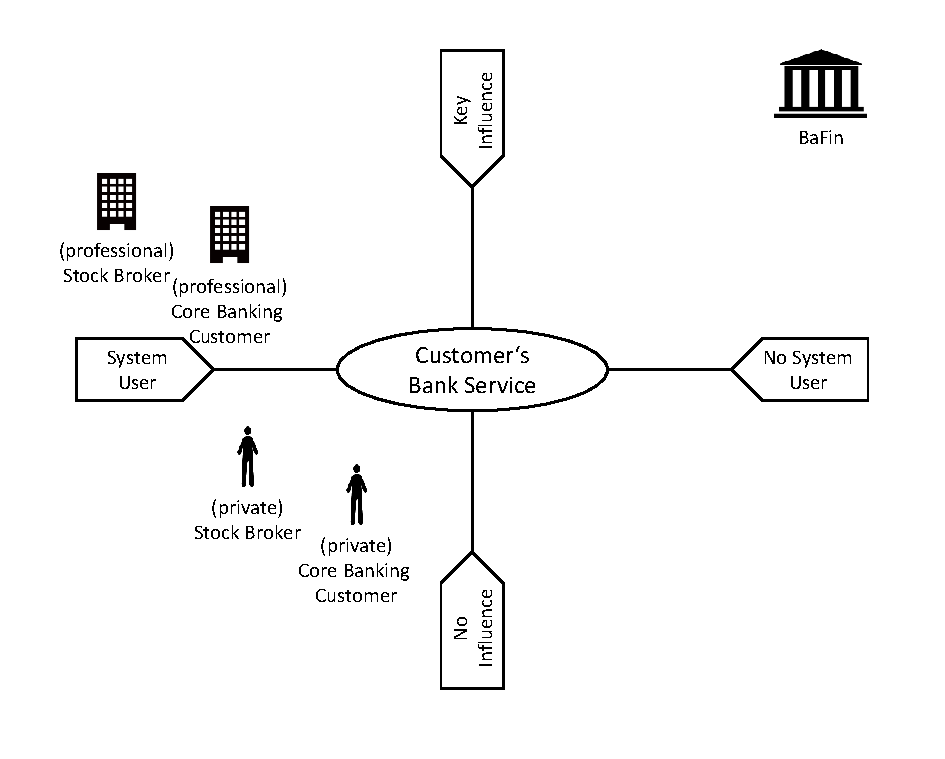
\includegraphics[height=.5\textheight]{img/smBank.pdf}
    \caption[Curate Bank Stakeholder Map]{Curate Bank Stakeholder Map (own illustration)}
    \label{fig:my_label}
\end{figure}

Regarded most influential, the BaFin is not using the banking service. This is certainly false for at least one bank since they have to transfer money as well as any other entity of the market. On the other hand, the BaFin will most certainly not have bank accounts at a major part of the banks operating in Germany. Second most influential are B2B stock trading customers. B2B customer do have more individual terms and conditions with the banks and can thereby make a huger impact on the bank's services. Stock trading customers do have a higher influence level due to the broader interaction with the bank. Therefore, the private customers rank fourth (stock trading) and fifth (core banking only).

\paragraph{} In terms of usage, stock brokers will be most likely to use the banking service more often, because they have more to do. Professionals will use the bank service more frequently than private individuals, because most companies turn over more money than companies. 

\subsubsection{Personas}
The complete set of personas can be seen in the appendix (cf. \cpagerefrange{}{}). As an exemplary case, follows the persona of Patrick Maurer, who is a procurement manager at a bank in Frankfurt. He is kind of a diligent and wary once it comes to marketing presentations. This is because as a procurement manager, he is being held responsible, if what he ordered was not what it promised to be. 

\begin{figure}
    \centering
    \includegraphics[]{}
    \caption[]{}
    \label{fig:}
\end{figure}

He would use the application, if it gave him quick insights into the suppliers skills. What he refuses to take a look into are marketing phrases, which contain no controllable information or arbitrary facts, anyone can find out without deeper knowledge of the banking industry. As requirements for the system, he uses a PC running Windows 7 for work and browses the web with the pre-installed Internet Explorer. Since his company checks every Update by Microsoft for Bug before delivering them to the employees, he is sometimes not on the newest Version of the Software. He does not use a smart phone, but a classic cellphone.

The personal traits were results of past experience of the author. The reasons Patrick gained the technical traits, was to fulfill the overall statistics, as follows:
\begin{enumerate}
    \item \textcite{StatCounter.2017} measured every tenth desktop user on the web uses Internet Explorer and 39\% used Windows 7. 
    \item In recent occasions it became clear that corporate IT-Infrastructure is updated by complicated procedures, which try to ensure compatibility, but delay update delivery drastically \parencites{Gierow.2017}{Zivadinovic.13.05.2017}.
\end{enumerate}

\subsection{Existing System Information}
As mentioned earlier, IBM require w3ID-Log in for employees, which is a OAuth2.0 \parencite[cf.][]{InternetEngineeringTaskForce.2012} based authentication procedure. This has to be fulfilled in order to have  usable product. 
\begin{closeItem}
    \item [
\end{closeItem}
\paragraph{}

\section{System Context Definition}
\subsection{Entities}

\subsection{IT-System}

\subsection{Usage}

\subsection{Development}


\section{Engineering Requirements}


\chapter{Discussion}


\chapter{Limitations and Future Work}


\chapter{Conclusion}